% Options for packages loaded elsewhere
\PassOptionsToPackage{unicode}{hyperref}
\PassOptionsToPackage{hyphens}{url}
%
\documentclass[
]{article}
\usepackage{lmodern}
\usepackage{amssymb,amsmath}
\usepackage{ifxetex,ifluatex}
\ifnum 0\ifxetex 1\fi\ifluatex 1\fi=0 % if pdftex
  \usepackage[T1]{fontenc}
  \usepackage[utf8]{inputenc}
  \usepackage{textcomp} % provide euro and other symbols
\else % if luatex or xetex
  \usepackage{unicode-math}
  \defaultfontfeatures{Scale=MatchLowercase}
  \defaultfontfeatures[\rmfamily]{Ligatures=TeX,Scale=1}
\fi
% Use upquote if available, for straight quotes in verbatim environments
\IfFileExists{upquote.sty}{\usepackage{upquote}}{}
\IfFileExists{microtype.sty}{% use microtype if available
  \usepackage[]{microtype}
  \UseMicrotypeSet[protrusion]{basicmath} % disable protrusion for tt fonts
}{}
\makeatletter
\@ifundefined{KOMAClassName}{% if non-KOMA class
  \IfFileExists{parskip.sty}{%
    \usepackage{parskip}
  }{% else
    \setlength{\parindent}{0pt}
    \setlength{\parskip}{6pt plus 2pt minus 1pt}}
}{% if KOMA class
  \KOMAoptions{parskip=half}}
\makeatother
\usepackage{xcolor}
\IfFileExists{xurl.sty}{\usepackage{xurl}}{} % add URL line breaks if available
\IfFileExists{bookmark.sty}{\usepackage{bookmark}}{\usepackage{hyperref}}
\hypersetup{
  pdftitle={Intro to Optimization},
  pdfauthor={Jake Underland},
  hidelinks,
  pdfcreator={LaTeX via pandoc}}
\urlstyle{same} % disable monospaced font for URLs
\usepackage[margin=1in]{geometry}
\usepackage{graphicx,grffile}
\makeatletter
\def\maxwidth{\ifdim\Gin@nat@width>\linewidth\linewidth\else\Gin@nat@width\fi}
\def\maxheight{\ifdim\Gin@nat@height>\textheight\textheight\else\Gin@nat@height\fi}
\makeatother
% Scale images if necessary, so that they will not overflow the page
% margins by default, and it is still possible to overwrite the defaults
% using explicit options in \includegraphics[width, height, ...]{}
\setkeys{Gin}{width=\maxwidth,height=\maxheight,keepaspectratio}
% Set default figure placement to htbp
\makeatletter
\def\fps@figure{htbp}
\makeatother
\setlength{\emergencystretch}{3em} % prevent overfull lines
\providecommand{\tightlist}{%
  \setlength{\itemsep}{0pt}\setlength{\parskip}{0pt}}
\setcounter{secnumdepth}{-\maxdimen} % remove section numbering
\usepackage{amsmath}
\usepackage{xcolor}

\title{Intro to Optimization}
\usepackage{etoolbox}
\makeatletter
\providecommand{\subtitle}[1]{% add subtitle to \maketitle
  \apptocmd{\@title}{\par {\large #1 \par}}{}{}
}
\makeatother
\subtitle{Optimization and Pattern Recognition Fall, 2021}
\author{Jake Underland}
\date{2021-10-05}

\begin{document}
\maketitle

{
\setcounter{tocdepth}{3}
\tableofcontents
}
\hypertarget{types-of-optimization}{%
\section{Types of Optimization}\label{types-of-optimization}}

\hypertarget{finding-extremums}{%
\subsection{Finding Extremums}\label{finding-extremums}}

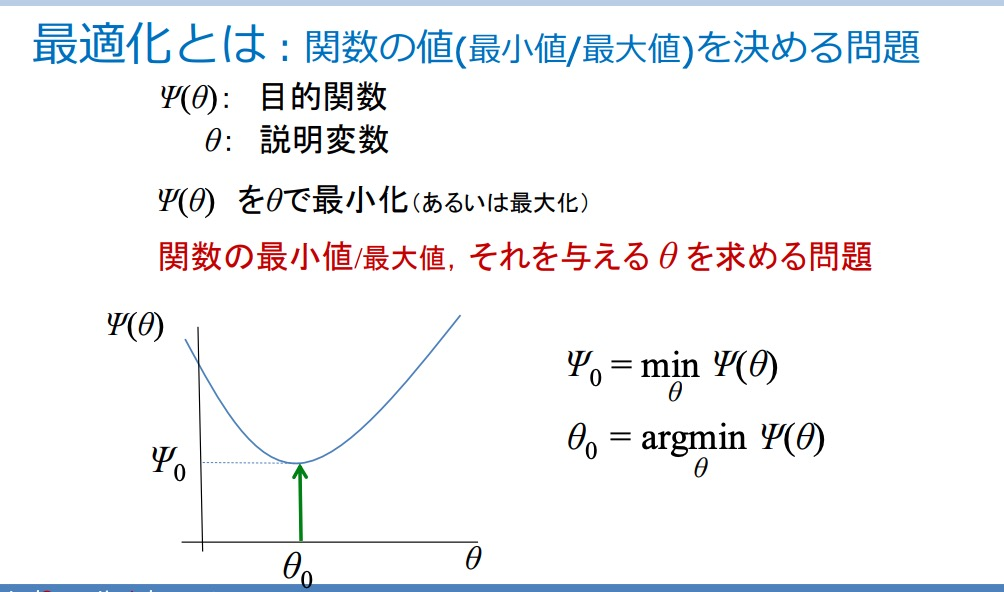
\includegraphics[width=\textwidth,height=0.4\textheight]{1.jpg}

\hypertarget{determining-shape-of-function}{%
\subsection{Determining Shape of
Function}\label{determining-shape-of-function}}

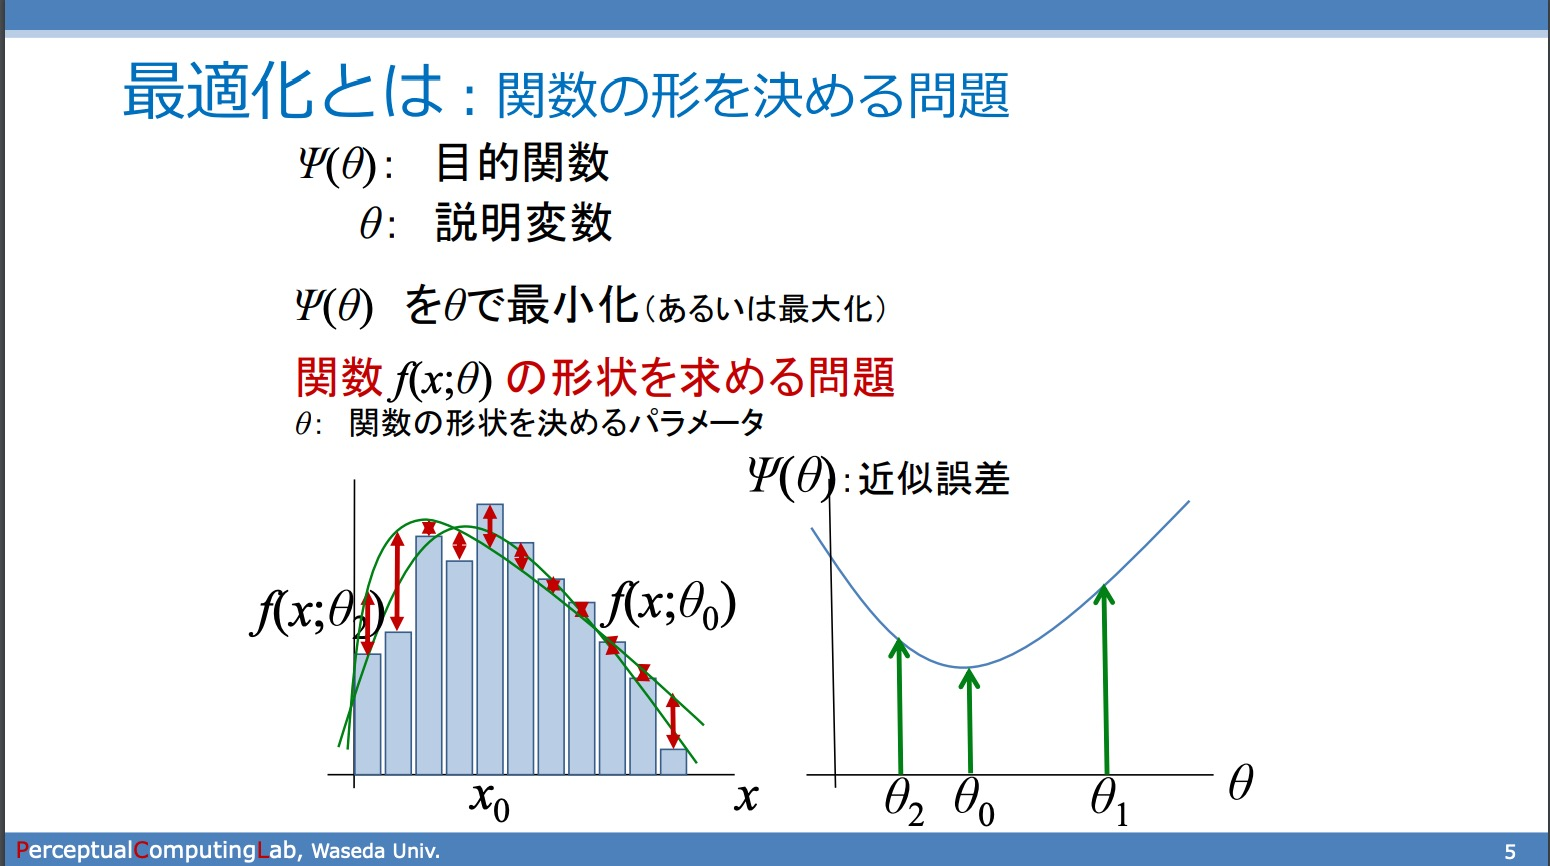
\includegraphics[width=\textwidth,height=0.4\textheight]{2.jpg} Find the
value of variable \(\theta_0\) such that the error function
\(\Psi(\theta)\) is minimized. Note that this optimization problem can
be translated into the first type (optimizing by finding extremums)
through the use of an error function. Many approximation problems make
use of this method.

\hypertarget{determining-optimal-sequence-in-sequential-decision-process}{%
\subsection{Determining Optimal Sequence in Sequential Decision
Process}\label{determining-optimal-sequence-in-sequential-decision-process}}

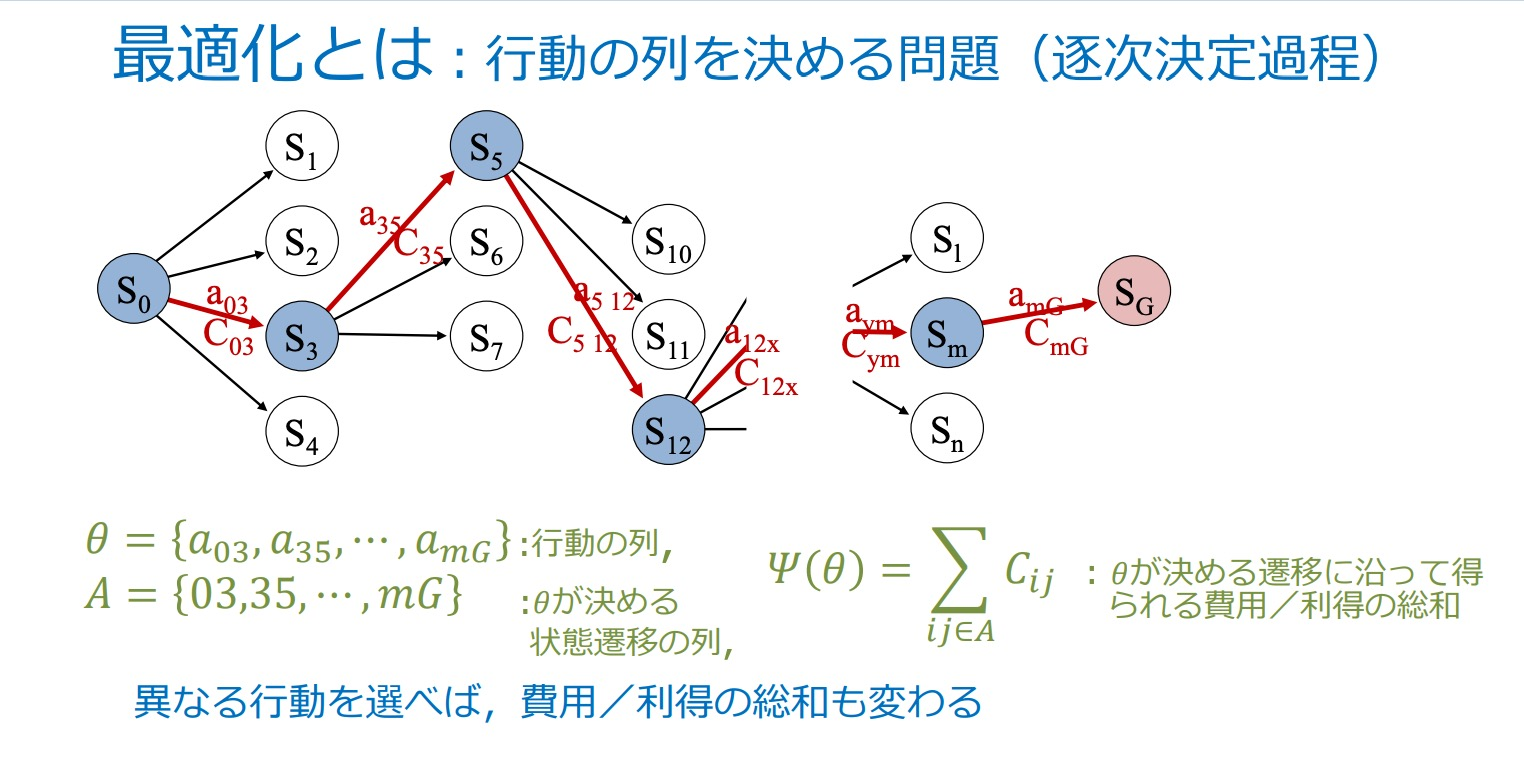
\includegraphics{3.jpg} \(\theta\) represents a sequence of actions,
\(A\) represents the sequence of states determined by \(\theta\), and
\(\Psi(\theta)\) is the cost of taking a certain \(\theta\), computed as
\(\sum_{ij\in A} C_{ij}\).

\hypertarget{formal-definition}{%
\section{Formal Definition}\label{formal-definition}}

\[\begin{aligned}
\Psi(\theta):& \text{ Objective (Target) Function} \\
\theta:& \text{ Explanatory Variable determining } \Psi
\end{aligned}\]

Optimization means to minimize (maximize) \(\Psi\) using \(\theta\).

\hypertarget{formal-characterization}{%
\section{Formal Characterization}\label{formal-characterization}}

\hypertarget{continuous-optimization}{%
\subsection{Continuous Optimization}\label{continuous-optimization}}

\begin{itemize}
\item \textbf{Nonlinear Programming Problem}: \newline
Includes nonlinearity in objective function or constraints. 
\begin{itemize}
\item \textit{Quadratic Programming Problem}: \newline
Objective function is a quadratic function, constraints are linear  
\item \textit{Convex Programming Problem}: \newline
Objective function is a convex function, area of constraint is convex
\end{itemize}
\item \textbf{Linear Programming Problem}: \newline
Objective function is linear, constraints are linear  
\end{itemize}

\hypertarget{discrete-optimization}{%
\subsection{Discrete Optimization}\label{discrete-optimization}}

\begin{itemize}
\item \textbf{Combinatorial Optimization Problem}  
\item \textbf{Integer Programming Problem}
\begin{itemize}
\item \textit{0-1 Integer Programming Problem:} \newline
Variables are either 0 or 1  
\end{itemize}
\end{itemize}

\hypertarget{application-example-facial-recognition}{%
\section{Application Example: Facial
Recognition}\label{application-example-facial-recognition}}

\[\begin{aligned}
\theta:& \text{ Model for Facial Features} \\
\Psi(\theta):& \text{ Pixel Error}
\end{aligned}\]

Begin by defining a model \(\theta\) for facial features. The one below
takes several prominent points of the face and connects them to form
triangles. Then, we can define the error function \(\Psi(\theta)\) to be
the squared sum of pixel differences; that is, if a triangle on the
training set captures black pixels but when applied to the testing set
captures beige pixels, that is computed as an error. Then, the
\(\theta\) that minimizes \(\Psi(\theta)\) provides us with a model for
the test data.\\
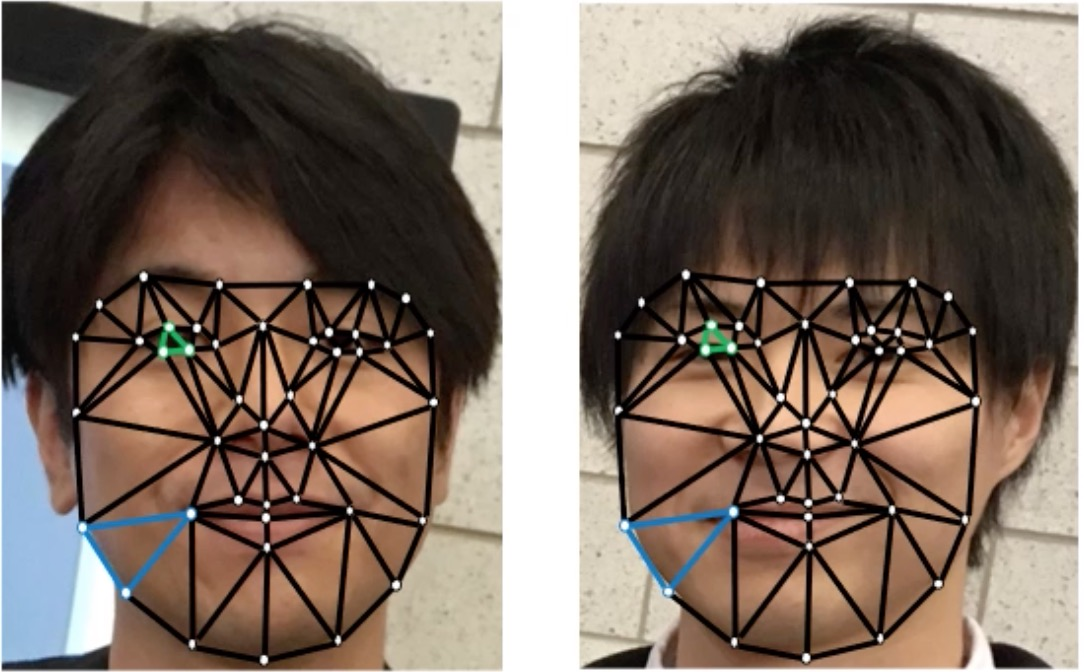
\includegraphics[width=0.5\textwidth,height=\textheight]{4.jpg}

\hypertarget{application-example-audio-source-separation}{%
\section{Application Example: Audio Source
Separation}\label{application-example-audio-source-separation}}

Two audio sources, two microphones, 4 paths (transformation functions)
for the audio to travel. We can reverse this filter by feeding it back
into the loop until each output audio sounds closer and closer to a
normal human being.\\
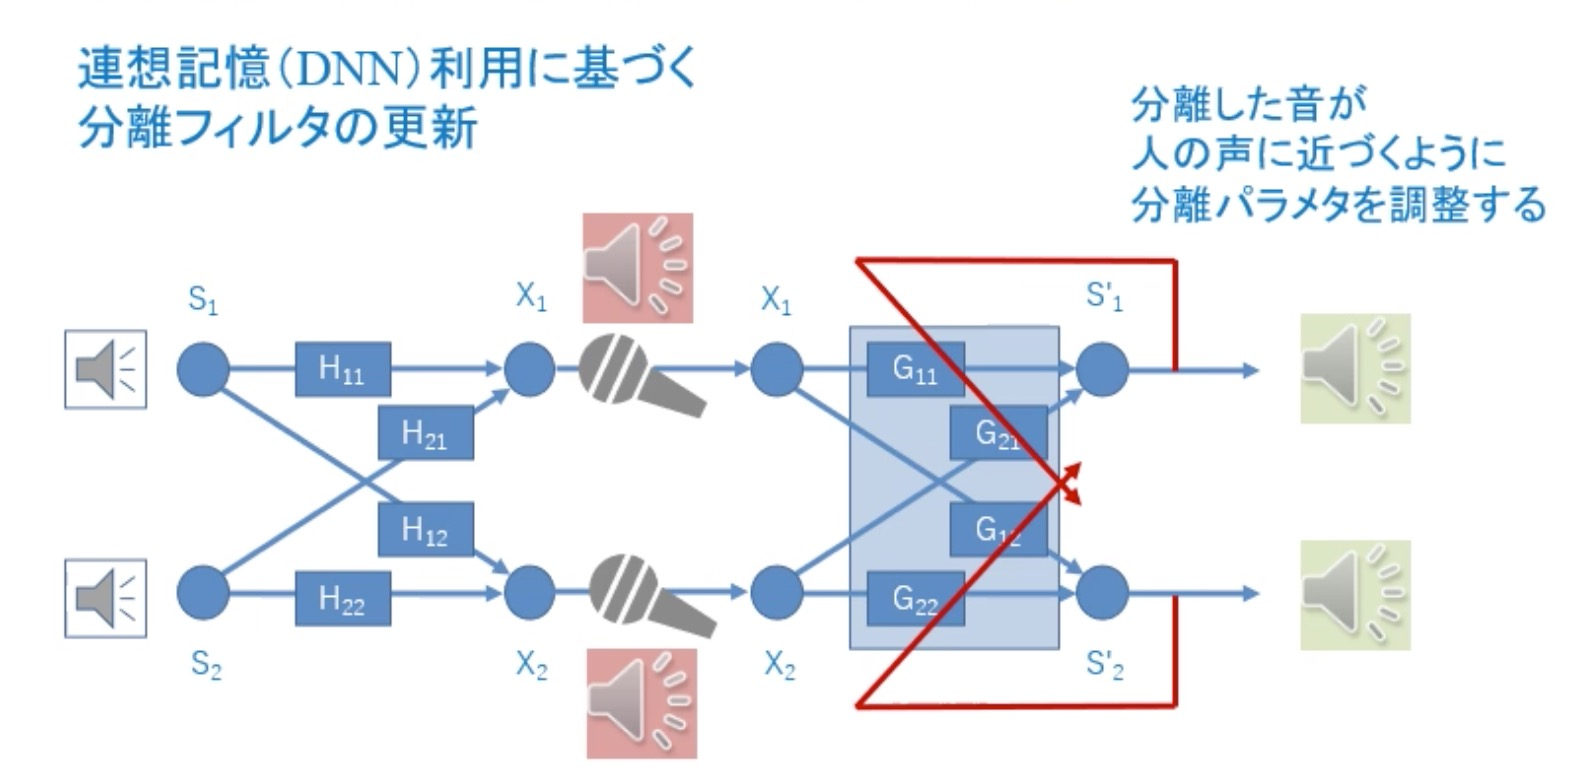
\includegraphics[width=0.7\textwidth,height=\textheight]{5.jpg}

\hypertarget{solving-continous-optimization-gradient-method}{%
\section{Solving Continous Optimization: Gradient
Method}\label{solving-continous-optimization-gradient-method}}

There is no analytic solution to continuous optimization, but one method
is to approximate an initial value and study the gradient in the
neighborhood of this value to arrive at the optimum.\\
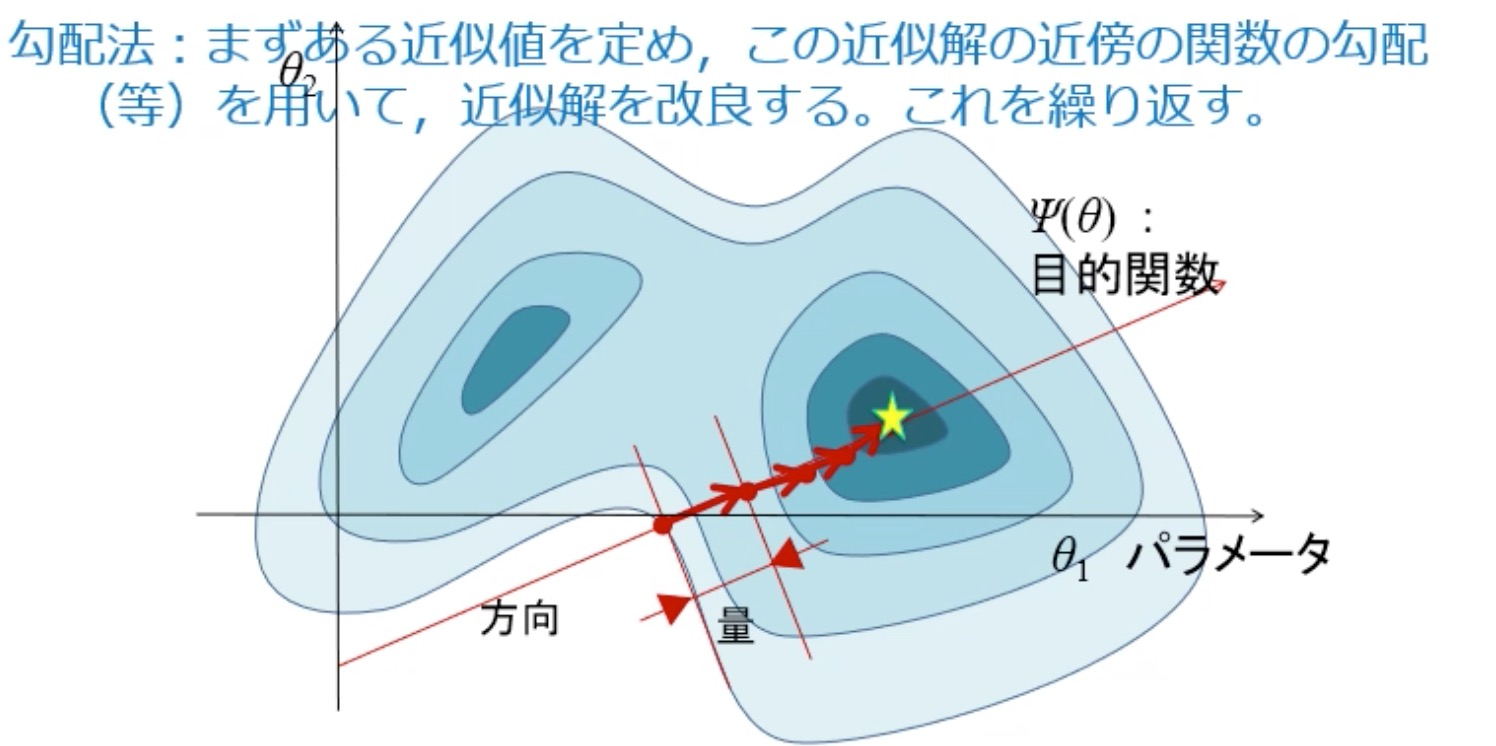
\includegraphics[width=0.7\textwidth,height=\textheight]{6.jpg}

We can add equality and inequality constraints of the parameters
\(\theta_1, \theta_2\) to the above:

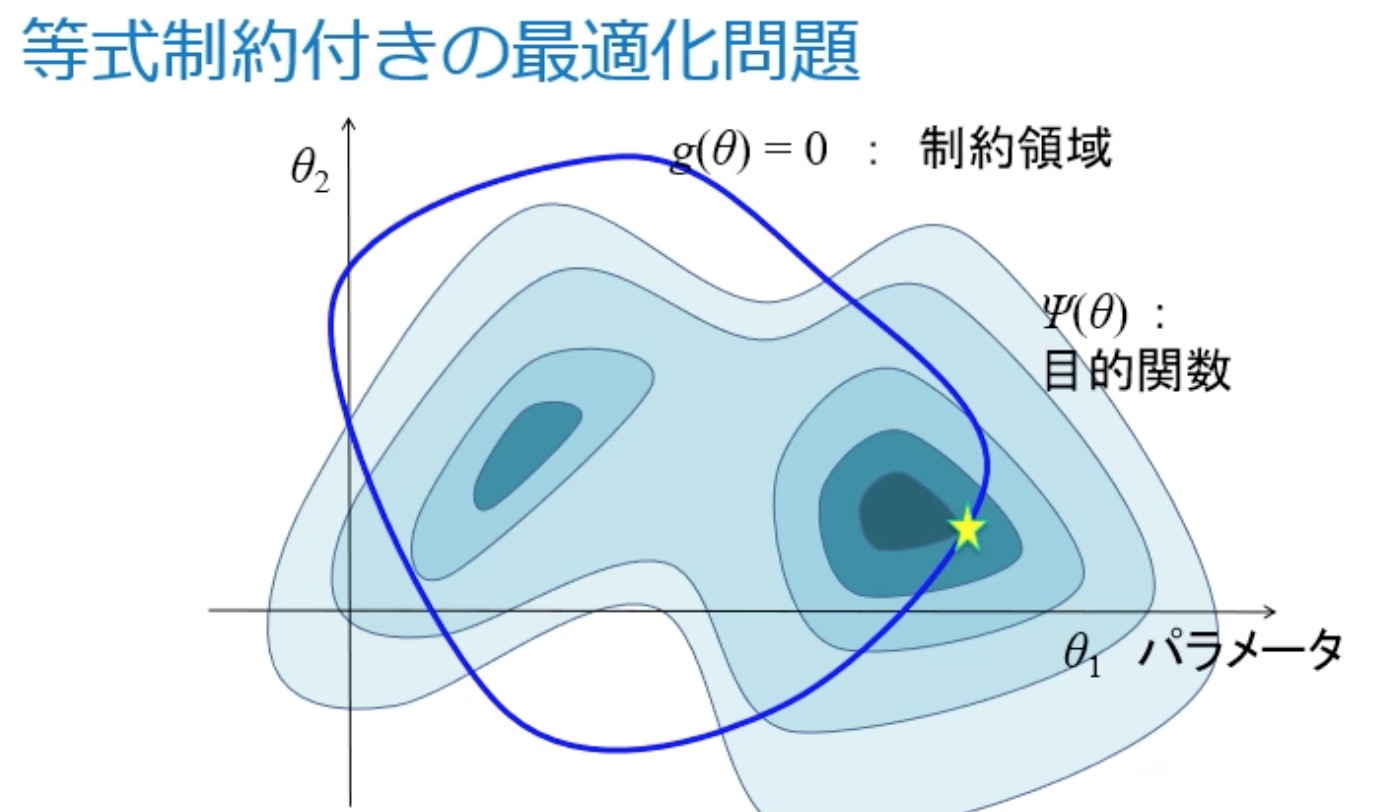
\includegraphics[width=0.5\textwidth,height=\textheight]{7.jpg}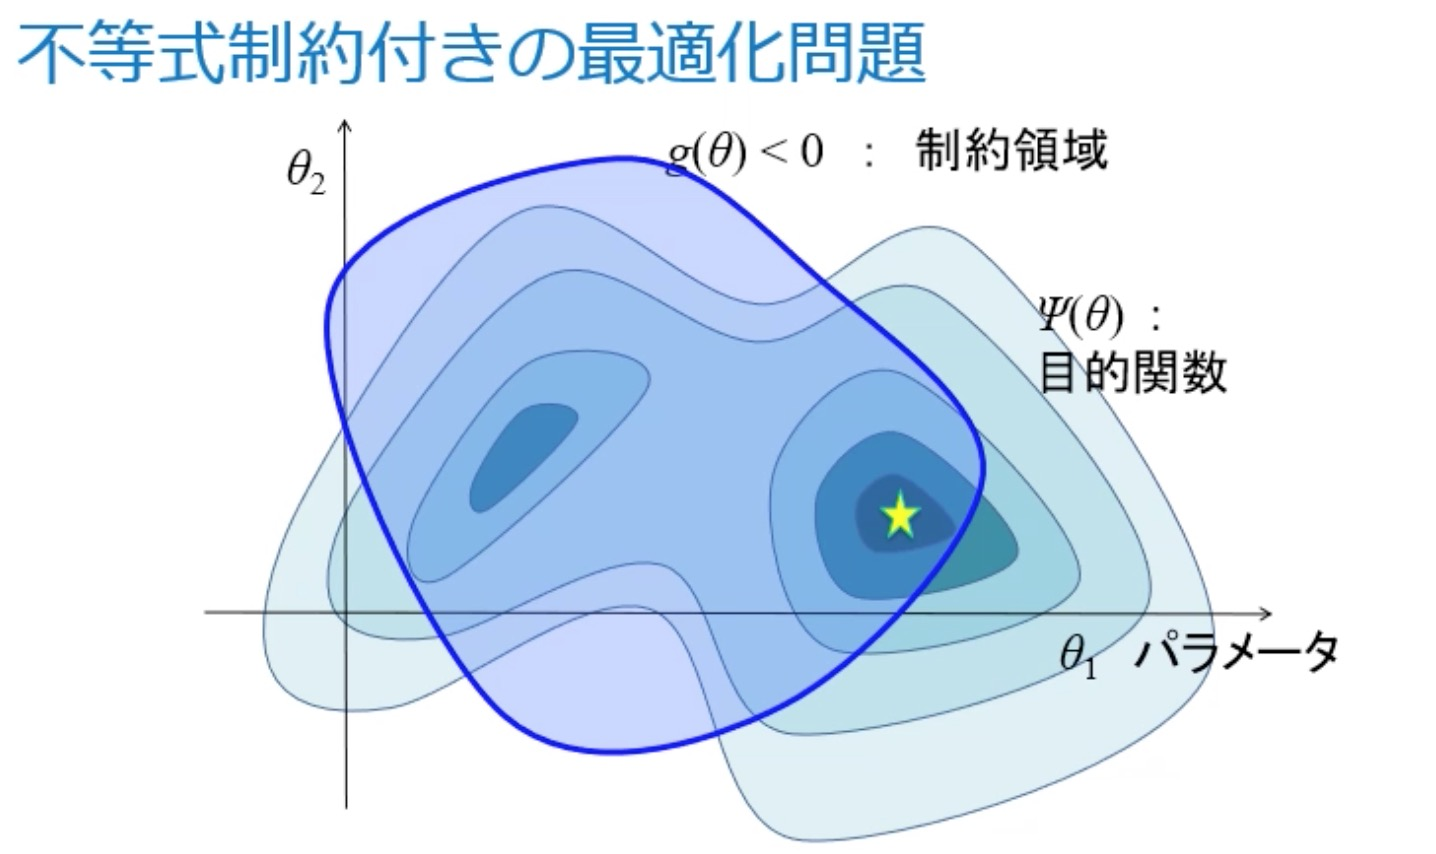
\includegraphics[width=0.5\textwidth,height=\textheight]{8.jpg}

\hypertarget{discrete-optimization-problems}{%
\section{Discrete Optimization
Problems:}\label{discrete-optimization-problems}}

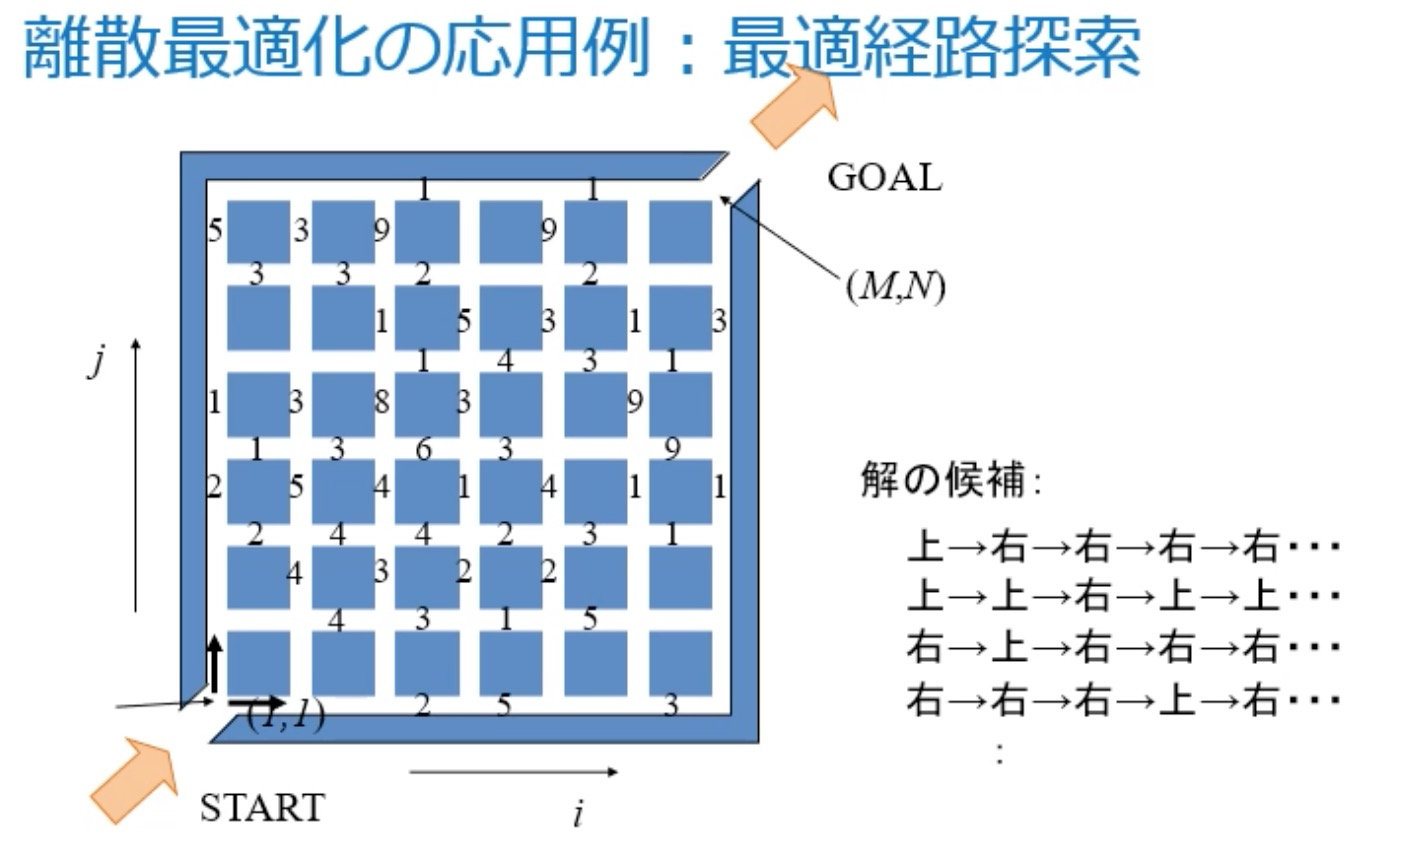
\includegraphics[width=0.5\textwidth,height=\textheight]{9.jpg}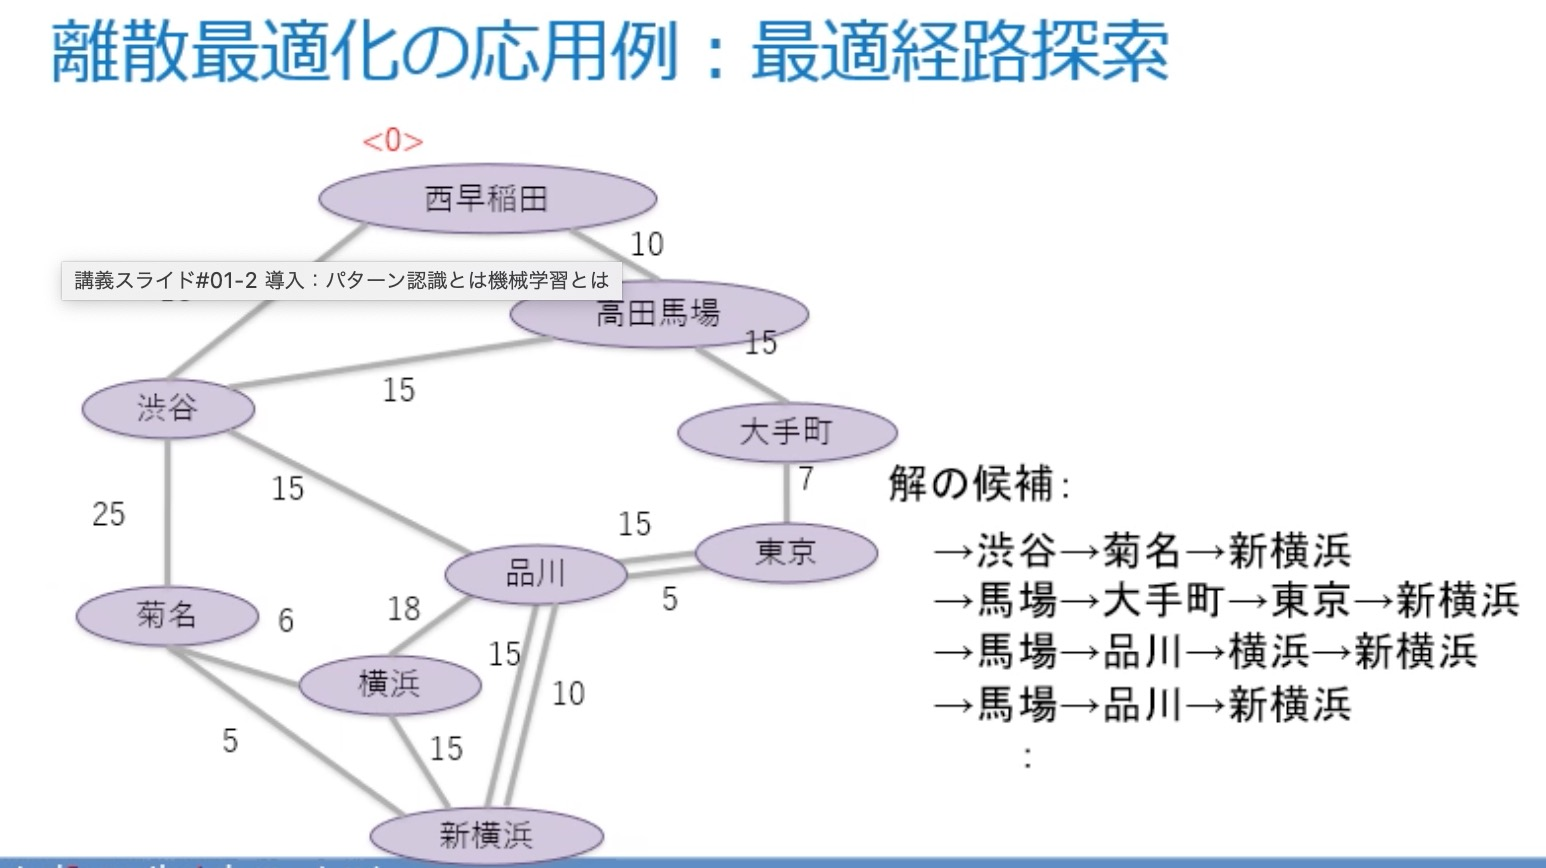
\includegraphics[width=0.5\textwidth,height=\textheight]{10.jpg}

\end{document}
